\documentclass{article}

% Language setting
% Replace `english' with e.g. `spanish' to change the document language
\usepackage[english]{babel}

% Set page size and margins
% Replace `letterpaper' with `a4paper' for UK/EU standard size
\usepackage[letterpaper,top=2cm,bottom=2cm,left=3cm,right=3cm,marginparwidth=1.75cm]{geometry}

% Useful packages
\usepackage{amsmath}
\usepackage{graphicx}
\usepackage[colorlinks=true, allcolors=blue]{hyperref}
\usepackage{placeins} % /FloatBarier

\title{Capstone project report -- Inventory Monitoring at Distribution Centers}
\author{Jakub Porebski}

\begin{document}
	\maketitle

\section{Project hyperlinks}
Useful links for the project description:
\begin{itemize}
	\item Github repository: \href{https://github.com/jakpor/Udacity-AWS-ML-project-5}{Udacity-AWS-ML-project-5}
	\item Project proposal document: \href{https://github.com/jakpor/Udacity-AWS-ML-project-5/blob/master/project_proposal/project_proposal.pdf}{project\_proposal/project\_proposal.pdf}
	\item Proposal review: \href{https://review.udacity.com/#!/reviews/3490974}{Review \#3490974}
\end{itemize}

\section{Project Overview}
In modern times logistics and delivery systems are crucial to various parts of the industry. Covid-19 pandemic showed that even short breaks in the logistics chain have huge consequences. Therefore, the big warehouses require reliable and automated system to sort and distribute packages based on multiple characteristics: delivery address, type of material. In these warehouses, packages/objects are usually carried over in boxes, where each box can hold multiple items. The task for the automated delivery system would be to classify the package and determine where to deliver it. But before that the system needs to know how many packages are in each delivery box and that will be the topic of the proposed Capstone project.

In order to count number of objects in a box I would like to make use of \href{https://registry.opendata.aws/amazon-bin-imagery/}{Amazon Bin Image Dataset}, which contain photo of the box content and other objects' characteristics including number of objects. Based on this image the implemented solution will estimate number of objects. 

Similar tasks for counting and characterizing objects in a box can be found in literature e.g. \href{https://arxiv.org/pdf/2107.04852.pdf}{''SynPick: A Dataset for Dynamic Bin Picking Scene Understanding''}

\section{Problem Definition}
In this Section I would like to define the problem to solve and investigate potential solutions and performance metrics.

\subsection{Goal of the project}
The main goal of the project is to create a solution for counting number of objects in each bin base on a photo of the bin’s content. The delivered model should have known accuracy in order to predict future false detection rate.

A solution of the project will be a ML model which will be able to determine number of objects in a box based on the photo of the box's content. For the delivered model accuracy will be computed in order to assess the model quality.

\subsection{The datasets and inputs}
For the project I used the \href{https://registry.opendata.aws/amazon-bin-imagery/}{Amazon Bin Image Dataset}. From this dataset I used only around 10000 images labeled with number of items inside a bin. Dataset will be post-processed and divided into train/valid and test subsets.

Amazon description of the dataset: ''The Amazon Bin Image Dataset contains over 500,000 images and metadata from bins of a pod in an operating Amazon Fulfillment Center. The bin images in this dataset are captured as robot units carry pods as part of normal Amazon Fulfillment Center operations.''

Selected subset of around 10000 objects are divided into three subsets for training, test and validation with ratios 60\%-20\%-20\% in corresponding sets. In the selected datasets number of images per class will be balanced, meaning for each class (number of objects in bin) there will be similar number of test/train/validation images. Balancing classes is needed to limit the bias effect in the result network.

\subsection{Strategy and realization plan}
The project requires classifying input images into multiple classes. I could be realized as an classical image processing and segmentation task, where each object is identified or using machine learning image classification network. As this Udacity course is focusing on ML application I will be implementing the latter option.

Machine learning requires a lot of resources in order to train the network for the task. I can use personal computer to complete computations or I could work on a cloud solution such as AWS. In this case much simpler solution would be to train the network locally and for the final training steps use cloud computing, however the nanodegree I am attending focuses on AWS cloud application therefore I would like to try my skills in that area. Cloud application offers user access to variety of computational machines and ease the process of deployment and integration of the model. Nevertheless, cloud interface seems to be in the state of continuous change. Tutorials used in the Udacity course are already outdated in many points, due to the fact that AWS added some new functions and upgraded user interface. 

Expected solution of the project will be a trained network model file which I could use to count number of objects in the delivery bin. 

\subsection{Baseline model selection}
As a baseline model I would like to use resnet50 image classification network. ResNet-50 is a convolutional neural network that is 50 layers deep. In AWS cloud there is available a pretrained version of the network trained on more than a million images from the \href{http://www.image-net.org}{ImageNet database}. The pretrained network can classify images into 1000 object categories, such as keyboard, mouse, pencil, and many animals. As a result, the network has learned rich feature representations for a wide range of images. The network has an image input size of 224-by-224.

Usage of the pretrained network is justified, because it limits the time needed to get accurate results and the pretrained network has higher change to generalize solution and work on new, not know data.

\subsection{Evaluation Metrics}
The quality of the training process will be evaluated using standard metrics: Cross Entropy Loss function and precision(accuracy). These metrics will measure and quantify the solution and ensure its repeatability for further improvements. For the training procedure a hyper parameter optimization might be needed to ensure that the training process will converge to expected result and won't over-fit to the dataset.

\section{Data analysis}
In this section I will present the overview of the dataset and analyse the problem through visualizations and data exploration to have a better understanding of what algorithms and features are appropriate for solving it.

\subsection{Dataset overview}
The Amazon Bin Image Dataset contains over 500,000 images and metadata from bins of a pod in an operating Amazon Fulfillment Center. In order to limit training time and AWS costs I used provided JSON file with list of 10441 images divided into 5 classes -- with number of items in range $\{1,2,3,4,5\}$.

Sample images from the dataset are presented in Figure~\ref{fig:samples}.
\begin{figure}[ht]
	\centering
	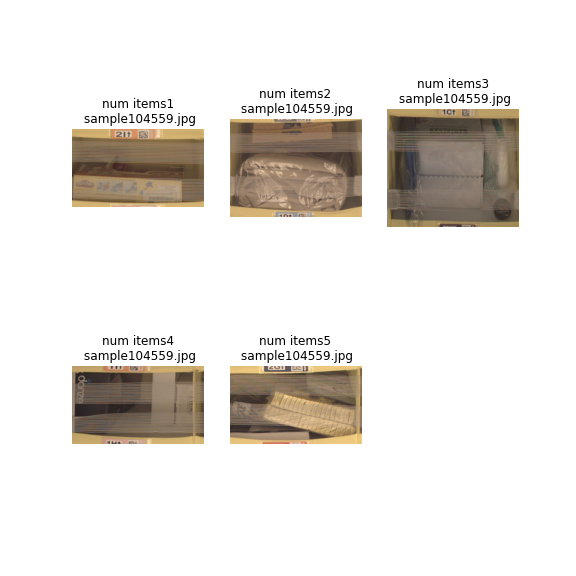
\includegraphics[height=90mm]{../project/sample_dataset_images.png}
	\caption{Sample images from the dataset}
	\label{fig:samples}
\end{figure}

As in the project we are dealing with only 5 classes, samples distribution can be represented as a list: 
\begin{itemize}
	\item Single object -- $1228$ images -- $12\%$ of the dataset,
	\item Two objects -- $2299$ images -- $22\%$ of the dataset,  
	\item Three objects -- $2666$ images -- $25\%$ of the dataset,  
	\item Four objects -- $2373$ images -- $23\%$ of the dataset,
	\item Five objects -- $1875$ images -- $18\%$ of the dataset,  
\end{itemize}
However for larger number of classes it would be best to represent the datased distribution in form on a histogram as presented in Figure~\ref{fig:histogram}.
\begin{figure}[ht]
	\centering
	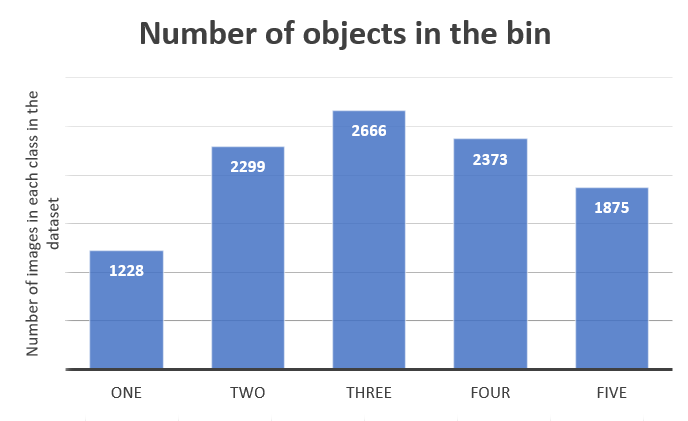
\includegraphics[height=60mm]{data_histogram.png}
	\caption{Histogram of the class distribution in used dataset.}
	\label{fig:histogram}
\end{figure}

Number of images for single and five objects in bin are a bit lower than other images, but each class has a representative contribution to the dataset. It is needed to ensure that the model will perform with constant accuracy regardless to the number of objects in bin. If the numbers deviated much more, the network might not generalize enough to distinguish each class in the dataset.

\FloatBarrier

\subsection{Model selection}
Task of this project is an image classification task. In order to complete it is the best to use pretrained image classification network, which already is able to process and classify some image data. I choose resnet50 network, because I am familiar with the input and output data structures of the network and it is easily available in pytotch models. Other image classification networks might be also appropriate for the task. 

\section{Model implementation}
The project is created in AWS domain using Sagemaker notebooks with some options to limit costs of future development and network training. 
Main steps of the project implementation consist of:
\begin{enumerate}
	\item Data preparation
	\begin{itemize}
		\item fetching data from a database, 
		\item pre-process data and divide it into test, train and validation subsets
		\item upload the data to S3 container
	\end{itemize}	
	\item Model tuning
	\begin{itemize}
		\item tune hyperparameters of the model
		\item train a machine learning model and observe if there are no anomalies in training.
		\item measure KPI metrics, plot training results
	\end{itemize}	
	\item Model deployment
	\begin{itemize}
		\item verify that the model is working as expected
		\item observe the quality of the outcome object
	\end{itemize}
\end{enumerate}
Each part of this procedure will be described in this section.

\subsection{Udacity project requirements}
This is the quote from the project definition in the Udacity course, which was completed in the current project.
\begin{quote}
	To finish this project, you will have to perform the following tasks:
	\begin{enumerate}
		\item Upload Training Data: First you will have to upload the training data to an S3 bucket.
		\item Model Training Script: Once you have done that, you will have to write a script to train a model on that dataset.
		\item Train in SageMaker: Finally, you will have to use SageMaker to run that training script and train your model
	\end{enumerate}
\end{quote}

\subsection{Data preparation}
The downloaded 10441 images had to be divided into train, test and validation subsets. For this project I divided images using 60-20-20 rule:
\begin{itemize}
	\item Train: 60\%
	\item Test: 20\%
	\item Valid: 40\%
\end{itemize}

The network accepts only RGB images with resolution $224\times224$ pixels therefore each image has to be resized and vectorized to match the input layer of the network.

\subsection{Data augmentation -- preprocessing steps}
In the distribution centers bins might be rotated and the network should be able to count the objects regardless of the box rotation. Therefore in the training process I apply random image flipping to ensure that the mirrored images will yield the same results in the network. 

Moreover the network should also count smaller and bigger objects in the bin. Therefore in the resize process I apply random image cropping to ensure that differently scaled images will present the same results.

Preprocessing steps applied:
\begin{itemize}
	\item Random image cropping -- from the original image randomly crop smaller image with size of $224\times224$px. This allows to artificially extend the training dataset and ensure that differently scaled images will present the same results.
	\item Random image flipping -- flip image horizontally, hence the network should be proof against different orientation of the bin or the objects within
	\item Data serialization -- 2D image had to be converted into 1D tensor of data in order to properly pass them to the model
\end{itemize}

I explicitly did not enable normalization of the color space for the images, because I was curious if model can operate and deduce the normalization factor by itself. This task was possible, because images from Amazon Bin Image Dataset are collected with similar lightning conditions and they are generally similar to each other if it comes to the color space. If I would like to estimate mean and standard deviation for the images it would be best to determine this information on a full dataset, which I did not want to download to fit in provided AWS costs per project.

\subsection{Hyperparameters tuning}
For the tuning procedure I started with a simplified script ''hpo.py'' which executes just a single epoch on a part of training data. This script was used to tune learning rate and batch size hyperparameters in following ranges:
\begin{itemize}
\item Learning rate was tuned for range: $(0.001, 0.1)$ - found optimal value is $0.0011430449671521476$.
\item Batch size was tuned for values: $\{32, 64, 128, 256, 512\}$ - found optimal value is $32$.
\end{itemize}

Hyper-parameter tuning was performed to search the 2D parameter space in the aforementioned ranges. Screenshot of the list of completed AWS jobs with their metric is presented in Figure~\ref{fig:hp_tuning}.
\begin{figure}[ht]
	\centering
	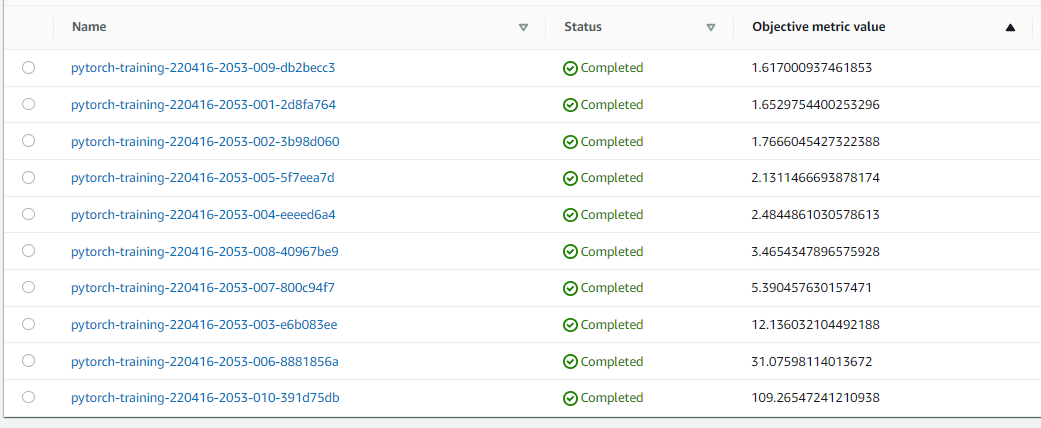
\includegraphics[height=50mm]{hp_tuning.png}
	\caption{List of hyper-parameter tuning jobs with output cross entropy metric value}
	\label{fig:hp_tuning}
\end{figure}

Each job represent some set of hyper-parameters and based on that we can display dependency of each hyper-parameter against the metric value as a mesh as presented in Figure~\ref{fig:hp_mesh}
\begin{figure}[ht]
	\centering
	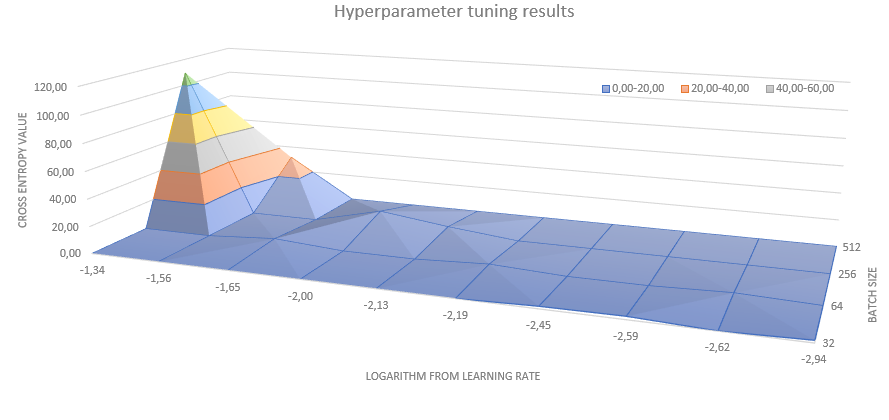
\includegraphics[height=80mm]{hp_mesh.png}
	\caption{Hyper-parameter value dependency to the training metric. Lower value the better.}
	\label{fig:hp_mesh}
\end{figure}

As we can observe in the hyper-parameter tuning plot -- Figure~\ref{fig:hp_mesh} -- for most of the tested samples the plot is quite flat. Based on that we can conclude that any value of learning rate below $0.01$ with any batch size would result in successful model training procedure. 

For the training I selected the best job's hyperparameters as a starting point: 
\begin{itemize}
	\item Learning rate: $0.001$
	\item Batch size: $32$
\end{itemize}

\subsection{Model training procedure}
After identification of potentially the best hyperparameters I ran training procedure for this task. The code for the training is provided in ''train.py'' file. The file is prepared to be working from Sagemaker notebook (example usage in ''sagemaker.ipynb'') or as a standalone script which can run on your personal machine or on low-cost spot instances. For the $10441$ files the training completed in $3$ epochs after $2$h of execution. Confirmation of the AWS job is presented in Figure~\ref{fig:model_tune}.
\begin{figure}[ht]
	\centering
	
\includegraphics[height=5mm]{model_tune.png}
	\caption{Snapshot of the tuned job in AWS cloud}
	\label{fig:model_tune}
\end{figure}

\section{Model training results}
The ''train.py'' file as prepared to be able to run from both SageMaker Instances and Spot Instances in AWS. In Sagemaker we can access multiple debugging tools to ensure that the training is progressing correctly, but the machines used there are costly. 

\subsection{Sagemaker Instance training}
I run the training in Sagemaker only for a part of the dataset and the Cross Entropy loss function is presented in Figure~\ref{fig:training_sage}.

\begin{figure}[ht]
	\centering
	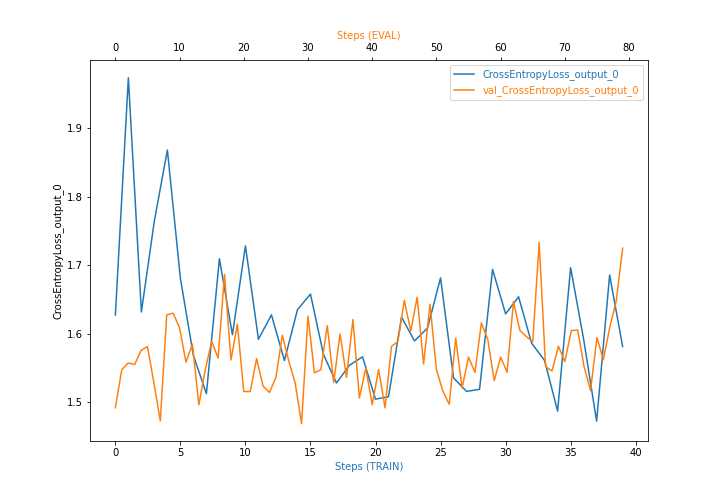
\includegraphics[height=80mm]{../project/training_debug_values.png}
	\caption{Cross entropy from Sagemaker training}
	\label{fig:training_sage}
\end{figure}

\subsection{Step Instance training}
However, for the full training I went to the ''Step instances'' in order to limit costs of the training process. In ''train.py'' file I have prepared debug prints which allowed me to visualize finalized training process. The same logs can be accessed in SageMaker using AWS CloudWatch service. Loss function and running accuracy plots are presented in Figures~\ref{fig:loss} and \ref{fig:acc} correspondingly.

\begin{figure}[ht]
	\centering
	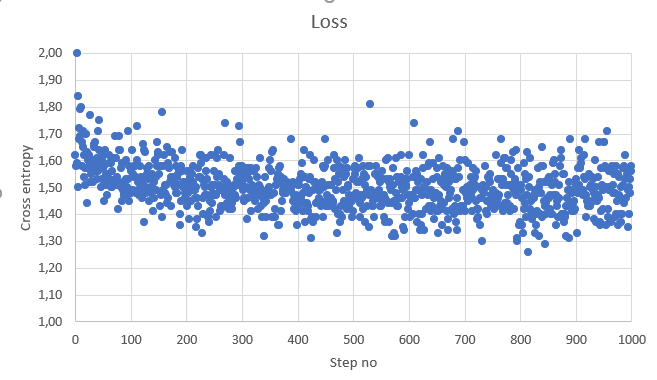
\includegraphics[height=80mm]{../project/loss.png}
	\caption{Cross entropy loss function changes during the training process.}
	\label{fig:loss}
\end{figure}

\begin{figure}[ht]
	\centering
	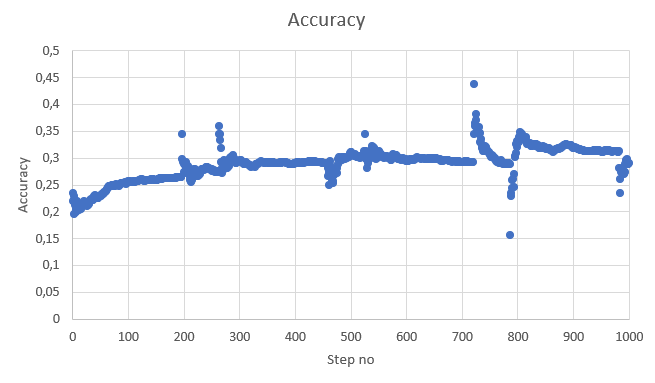
\includegraphics[height=80mm]{../project/accuracy.png}
	\caption{Running accuracy of the model through the training}
	\label{fig:acc}
\end{figure}

\FloatBarrier
\subsection{Model deployment}
After generating the trained I heve deployed it as Sagemaker Endpoint and tested it operation on a sample image. For the model inference I have created "inference.py" script, which can be used from Lambda or Sagemaker in AWS. Example code how to deploy the project and run sample inference is provided in ''sagemaker.ipynb'' notebook.

\subsection{Comparison of different pre-trained models}
In order to compare results between different jobs I trained the network using some different hyperparameter configuration in order to observe how models might behave differently.

For comparison, I trained network using:
\begin{itemize}
	\item Learning rate: $0.2$
	\item Batch size: $32$
\end{itemize}
Based on hyperparameters training job I could expect that this model will behave poorly as the learning rates $> 0.01$ were rejected by the tuning procedure.

The trained model failed after just two epochs with the error that the model loss started increasing between epochs.
The accuracy plot is presented in Figure~\ref{fig:acc2}.
\begin{figure}[ht]
	\centering
	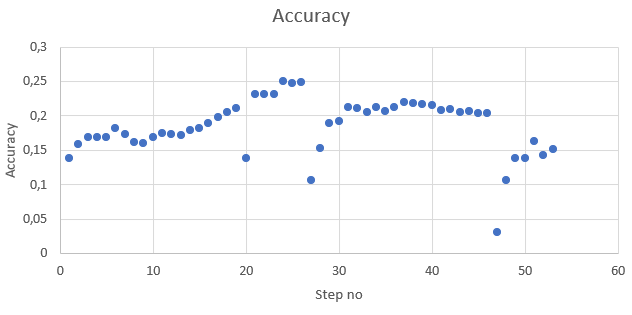
\includegraphics[height=80mm]{accuracy_bad.png}
	\caption{Running accuracy of the additional model for comparison}
	\label{fig:acc2}
\end{figure}

The comparative results show that in fact this model is producing less accurate results than the reference model with tuned hyperparameters (see Figure~\ref{fig:acc} for comparison). 

\section{Conclusions}
The final accuracy of the trained model is about $0.3$, which is not the best result. However, considering the fact that I used 5\% of the Amazon Bin Images Dataset and limited the training process to minimum, achieved accuracy is acceptable. In order to improve it however, training on a bigger part of the dataset should be performed. 

Comparison with the additional models showed that the hyperparameter tuning step was performed properly and the selected hyperparameter values are acceptable for further development. This also shows the importance of the hyperparameter tuning step and implies that even small search might produce significantly better outcome on the trained model.

Nevertheless, developed model for the task of counting objects in bin is not sufficient to effectively solve the stated problem. With accuracy of $0.3$ model will produce only $30\%$ of correct measurements, while $70\%$ of the bins will be classified incorrectly. As mentioned in the project specification, this model might act as a verification tool for other complex networks, which characterize more detailed objects parameters - colors, size, label, etc. For that purpose desired model accuracy should be quite high in order to cross-check other components in the system. In odrer to improve the model I would suggest training the model on a bigger part of the dataset and probably enable training even if the overall loss function is growing. In optimization techniques there is a method called ''annealing'', which might temporarily increase object entropy allowing it to decrease more than before.

During this project I learned how to use AWS cloud to deploy ML solutions following steps:
\begin{enumerate}
	\item Download dataset, preprocess it and store in S3,
	\item Train the network using Sagemaker and Spot istances
	\item Deploy a model as an endpoint and run inference on the model.
\end{enumerate}

\end{document}